% Template for Degree Programme in Computer Science and Engineering Diploma Thesis v1.3.2019
% Authors: Mika Korhonen (original author), Pekka Pietikäinen, Christian Wieser, Teemu Tokola, Juha Kylmänen, Tuomas Holmberg and Tuomas Varanka.
% If you make any improvements to this template, please contact teemu.tokola@oulu.fi
%
% CHANGELOG
% 2023-01-31: Track changes has been turned on - TTo
% 2023-06-15: Improvements to avoid missing filling in some details: TODO's added to template (TTo)
% 2023-06-15: Changes to foreword, clarifications to indicate template is also for Bachelor thesis  (TTo)
% 2023-06-15: Example of a CC-BY figure added with reference in the footnotes (TTo)


\documentclass[finnish]{csethesis}

\usepackage[type={CC}, modifier={by}, version={4.0}]{doclicense-csetemplate}

\copyrighttext
  {Copyright \textcopyright\ \number\year\ \getauthorslist. Except otherwise noted, the reuse of this document is authorized under a Creative Commons 4.0 International (CC-BY-4.0) license.}
  {%
    \textcopyright{}
    \number\year\ \getauthorslist.\par
    \doclicenseThis % CC logo, needs transparency removed
    Exception: The figures  are not included in the license.
  }
  
% Abstracts are placed in the metadata of the PDF file, 
% so they cannot contain empty lines or special characters.
% Mathematic symbols should be fine (mathxmp option for pdfx package),
\abstract{This document provides general guidance for a degree student
  of Computer Science and Engineering in preparing his/her master's
  thesis. This guide defines the role of a thesis in the
  M.Sc. Degree, presents the actions to be taken in different phases
  of the thesis procedure and introduces the way that master’s thesis
  is written. The document has been formatted based on these
  guidelines to serve as an example how the thesis should look like.}

\tiivistelma{Näissä ohjeissa opastetaan valmistumisvaiheessa olevaa
  opiskelijaa diplomityön tekemisessä. Ohjeissa selvitetään työn asema
  diplomi-insinööritutkinnossa, kerrotaan toimenpiteet, joihin työn
  tekijän on ryhdyttävä työn eri vaiheissa, sekä määritellään
  yksityiskohtaisesti diplomityön kirjallinen rakenne. Ohje on
  muotoiltu noudattaen näitä kirjoitusohjeita ja toimii siten
  esimerkkinä, miltä diplomityön tulisi näyttää.}

% Keywords are also included in the PDF metadata, and cannot contain any
% special characters. Separate them with \spc

\keywords{M.Sc. degree\spc master’s thesis instructions\spc structure of a master’s thesis}
\avainsanat{diplomi-insinöörin tutkinto\spc diplomityön ohjeet\spc diplomityön rakenne}

%%%%%%%%%%%%%%%%%%%%% SET YOUR INFORMATION HERE %%%%%%%%%%%%%%%%%%%%%%%
%%%%%%%%%%%%%%%%%%%%%%%%%%%%%%%%%%%%%%%%%%%%%%%%%%%%%%%%%%%%%%%%%%%%%%%%%
\title{TODO: Bachelor's and Diploma Thesis Guide}
\otsikko{TODO: Kandidaatintyön ja diplomityön teko-ohjeet}

\firstname{Author}
\lastname{One}

% Please choose the correct type of thesis and the language used
\thesis{Master} % {Bachelor | Master}

%Names of other authors can be added here
\firstnametwo{Author}
\lastnametwo{Two}
\firstnamethree{Author}
\lastnamethree{Three}
%Do not remove or comment the extra names if you do not need them, leave them empty instead


%%%%%%%%%%%%%%%%%%%%%%%%%%%%%%%%%%%%%%%%%%%%%%%%%%%%%%%%%%%%%%%%%%%%%%%%%
%%%%%%%%%%%%%%%%%%%%%%%%%%%%%%%%%%%%%%%%%%%%%%%%%%%%%%%%%%%%%%%%%%%%%%%%%
%\headertitlecap automatically creates headers with TitleCaps (Capitalizes the First Letter in Each Word) for H0, H2, and H3. Words not to be capitalized can be changed in di.sty
\headertitlecap

% Add your bibliographies here. You can use several
\addbibresource{citations.bib}

\begin{document}

\hypersetup{pageanchor=false}
\maketitlepage
    \pagenumbering{arabic}
    \setcounter{page}{1}
    \hypersetup{pageanchor=true}
    \makecopyrightpage{}
  
    \IfLang{\MainLang}{finnish}{
      \selectlanguage{finnish}

\begin{tiivistelma}

Näissä ohjeissa opastetaan valmistumisvaiheessa olevaa opiskelijaa diplomityön tekemisessä. Ohjeissa selvitetään työn asema diplomi-insinööritutkinnossa, kerrotaan toimenpiteet, joihin työn tekijän on ryhdyttävä työn eri vaiheissa, sekä määritellään yksityiskohtaisesti diplomityön kirjallinen rakenne. Ohje on muotoiltu noudattaen näitä kirjoitusohjeita ja toimii siten esimerkkinä, miltä diplomityön tulisi näyttää.

\avainsanat diplomi-insinöörin tutkinto, opinnäytetyön ohjeet, diplomityön
rakenne\footnote{Käytä avainsanoina eri sanoja kuin lopputyön otsikossa. Poista tämä alaviite lopputyöstäsi.}

%\avainsanat diplomi-insinöörin tutkinto, opinnäytetyön ohjeet, diplomityön
%rakenne.}

\end{tiivistelma}

\ifthenelse{\equal{\getlanguage}{english}}
    {\selectlanguage{english}}
    {}


      This document provides general guidance for a degree student of Computer Science and Engineering in preparing his/her master's thesis. This guide defines the role of a thesis in the M.Sc. Degree, presents the actions to be taken in different phases of the thesis procedure and introduces the way that master’s thesis is written. The document has been formatted based on these guidelines to serve as an example how the thesis should look like.

      \selectlanguage{finnish}
    } {
      This document provides general guidance for a degree student of Computer Science and Engineering in preparing his/her master's thesis. This guide defines the role of a thesis in the M.Sc. Degree, presents the actions to be taken in different phases of the thesis procedure and introduces the way that master’s thesis is written. The document has been formatted based on these guidelines to serve as an example how the thesis should look like.

      \selectlanguage{finnish}

\begin{tiivistelma}

Näissä ohjeissa opastetaan valmistumisvaiheessa olevaa opiskelijaa diplomityön tekemisessä. Ohjeissa selvitetään työn asema diplomi-insinööritutkinnossa, kerrotaan toimenpiteet, joihin työn tekijän on ryhdyttävä työn eri vaiheissa, sekä määritellään yksityiskohtaisesti diplomityön kirjallinen rakenne. Ohje on muotoiltu noudattaen näitä kirjoitusohjeita ja toimii siten esimerkkinä, miltä diplomityön tulisi näyttää.

\avainsanat diplomi-insinöörin tutkinto, opinnäytetyön ohjeet, diplomityön
rakenne\footnote{Käytä avainsanoina eri sanoja kuin lopputyön otsikossa. Poista tämä alaviite lopputyöstäsi.}

%\avainsanat diplomi-insinöörin tutkinto, opinnäytetyön ohjeet, diplomityön
%rakenne.}

\end{tiivistelma}

\ifthenelse{\equal{\getlanguage}{english}}
    {\selectlanguage{english}}
    {}


      \selectlanguage{english}
    }
    \contents %Insert table of contents
    \thispagestyle{empty}
\header{\headerforeword}
These guidelines are based on thesis instructions of the former Department of Electrical and Information Engineering, the instructions of the publication series Acta Universitatis Fennica, and the book “Teknisen kirjoituksen laatiminen” \cite{lappalainen, acta, tirronen}. Several persons from the former Department of Electrical and Information Engineering have participated in setting up these instructions. The preparation of the first version was led by Prof. Pentti Lappalainen.

The Finnish guidelines were edited by the Study Committee of the Department of Electrical and Information Engineering in 2005 and 2010-2011, and revised by the Degree Programme Committee of Computer Science and Engineering in 2011 and 2012. The original English version was written by the Degree Programme Committee of Electrical Engineering; this version is based on that version and the Finnish instructions for Computer Science and Engineering. This English version has been updated to comply with the new conventions for archiving the electronic versions of master’s theses in 2013, and the organization renewal in 2016 where the Department of Computer Science and Engineering was disbanded and divided into three research units. 

The instructions were revised in July 2018 for the Faculty of Information Technology and Electrical Engineering. The update was coupled with the transition to Overleaf as recommended \LaTeX\ document preparation platform. The key modification was the overhaul of referencing to IEEE style. This document is applicable for Bachelor's and Diploma theses completed in and after 2018.

The latest revisions in 2023 were made by the Computer Engineering Degree Program Committee to improve instructions and to clarify the use of footnotes and references in case of pictures.

\signature

    \header{\headerabbreviations}
\setlongtables
% According to updated thesis guidelines, lowercase Greek letters used as quantities
% are italicized. Uppercase Greek letters are upright.
\begin{longtable}[l]{p{3cm}p{0.7\textwidth}}

    CSE\footnote{Even though a symbol or an abbreviation is explained on this page, it should be written out full when appearing in the text for the first time. Remove this footnote from your thesis.} & Computer Science and Engineering\\
    GUI & graphical user interface\\
    LBP & local binary pattern\\
    NCC & normalized cross-correlation\\
    SVM & support vector machine\\
    UML & unified modeling language \\
    \\
    \textit{f} & focal length\\
    \textit{N} & number of samples\\
    \textbf{Q} & orthogonal matrix \\
    \textit{r\textsubscript{ij}} & matrix element \\
    \textit{s} & distance \\
    \textit{t} & time \\
    \textit{v} & velocity \\
    \textbf{v} & velocity vector \\
    \textbf{x} & planar coordinate \\
    \\
    $\beta$ & shape factor \\
    $\epsilon$\textsubscript{k} & error signal at instant k \\
    $\Phi$\textsubscript{k} & state transition matrix at instant k \\
    $\boldsymbol{\theta}$ & parameter vector \\
    $\sigma$\textsuperscript{2} & variance \\
    \\
    $\lfloor$ $\rfloor$ & integer part \\
    $\oplus$ & logical XOR operation \\
    $\arg$() & argument \\

\end{longtable}
\setcounter{table}{0}


    
    %sets the dots for numbered chapters in table of contents
    \addtocontents{toc}{\protect\renewcommand{\protect\cftchapleader}{\protect\cftdotfill{\cftdotsep}}}

    \chapter{Introduction} %Set the name of a new chapter
        \label{introduction} %Create a label for referencing purposes (\charef{.})
        \pagenumbers
        Writing a thesis takes on a major part of completing the master’s degree studies. The thesis assignment prepares for the independent engineering work. Hence, supervision plays a smaller role in thesis procedure than during previous studies. A typical master’s thesis represents a solution to a relatively extensive technical problem. Additional studies in the given field are often necessary; however, the aim of the thesis work is to make use of the knowledge and skills acquired during preceding studies. Furthermore, technical and scientific documentation skills will be strengthened. The thesis work can be a conducted as a part of a larger project, but the master’s thesis itself should be written individually.

The thesis work is undertaken in the final phase of the studies. It is recommended to begin the thesis work during the autumn term of the 2\textsuperscript{nd} study year in the master’s programme or the 5\textsuperscript{th} year after starting in the bachelor’s programme. However, timing is flexible and it is also possible to begin earlier depending on advancement in studies. As a general rule, it is time to get started, when there are 15 to 30 credit points left of the total coursework (in addition to the master’s thesis). Some fields of study require certain courses to be completed before the master’s thesis. Requirements should always be checked in advance with the supervisor. Information on the degree specific requirements is provided by the secretary of the degree program and the registered credit points can be viewed in Peppi.

\section{Thesis guide}
The aim of these instructions is to give detailed guidelines for composing and writing a master’s thesis. This document describes the thesis work process; starting from searching the topic to the formal approval of the completed thesis. The process has otherwise stayed the same for quite a while, but the final stages were changed in the beginning of 2013 due to electronic archiving for all master’s theses at the University of Oulu. Hence, the older versions of this document are no longer valid and should not be used. Moreover, this document offers practical instructions for the writing of the thesis: for the literary structure, the layout, and for the writing process as well. This document itself has been edited according to the instructed layout, though the literary structure is not similar to that of a master’s thesis.

Before starting your master’s thesis work, \textbf{please first read this document carefully.} Following these instructions closely is likely to produce a better result and a higher grade. When the supervisor does not have to point out about these instructions (specifically about the layout) she/he can focus on instructing on the content and how the best grades can be achieved. The degree programme web pages \cite{mscstudies} offer instructions for master thesis as well. When neither of these sources gives an answer to your questions, please ask your supervisor or from the study affairs office. And remember: Although writing the thesis can be difficult at times, every M.Sc. graduated from Faculty of ITEE has succeeded in this effort!

\section{Author's Contributions and the Role of Artificial Intelligence}

The structure of a thesis can vary. However, at the end of the introductory chapter, you must include a section titled \textit{Author's Contributions and the Role of Artificial Intelligence}. In this section, you should clarify your independent contributions to the thesis and explain how AI was used in its preparation, if applicable. More information can be found in Sections \ref{writing} and \ref{AI}.
 %Input the contents of the chapter from a separate file
    
    \chapter{General outline for thesis projects}
        \label{relatedwork}
        The process starts with specifying the topic of the thesis and applying for its formal approval by the degree programme committee head. You need to define the topic together with the commissioner and the supervisors (see the next section). The topic, commissioner, and supervisors are specified in the topic application form that is used to apply the approval of the topic. The list below presents the general thesis process, with emphasis on the administrative issues and supervision:

\begin{enumerate}
    \setlength\itemsep{0pt}
    \setlength\parskip{0pt}
    \item approval for the topic,
    \item writing the thesis (preferably at the same time as carrying out the research),
    \item delivering the thesis and applying for the degree,
    \item evaluation and grading, and
    \item granting the degree.
\end{enumerate}

The second stage is the most laborious part, which includes writing the thesis and performing the actual work, for example, designing, building and testing a piece of software. When the thesis is ready, it is reviewed by the supervisors, modified by you if necessary, and then delivered to the Laturi system. The next step is to apply for the degree certificate and to perform the other tasks that are required from graduating students. The supervisors download the thesis from the archive and evaluate it. The degree programme committee approves the grading in its meeting and the faculty grants the degree. The thesis is transferred to the university archive and published according to the publicity level you defined when uploading the thesis to Laturi. The graduation ceremony ends your M.Sc. studies. The process is explained in more detail in the rest of this document and on the degree programme web pages \cite{mscstudies}.

\section{Approval of the topic}

Your first task is to find a commissioner for your thesis that is typically a company which hires you to make a thesis project. For example, a summer job or training in a company or some other organization gives a good starting point to continue in a thesis project. A research unit in the Faculty of Information Technology and Electrical Engineering can also act as the commissioner, in which case the topic will most likely be linked with ongoing research at the unit. Research units provide information about current master’s thesis topics in their web pages. You can also directly ask topics from the research unit personnel. In some cases the research units can pay salary to the master’s thesis worker, but in most cases you need to be prepared to make the thesis for free.

There are 2-3 supervisors involved in the master’s thesis process, and they are assigned after the topic is confirmed. \textit{Principal supervisor} is a professor or a  doctor who belongs to the personnel of some ITEE research unit. A list of potential supervisors and their fields of expertise can be found from the degree program web pages \cite{mscstudies}. The professor or doctor you approach first can decide based on  the thesis topic to act as a principal supervisor her/himself or suggest someone else.  Usually, the thesis is done on a topic within the area of your orientation (major).  However, topics proposed by companies are often multi-disciplinary or cross-scientific  and the topic does not fit into the realm of any particular orientation. In these cases  the supervision should be agreed with a professor or doctor who best represents the  overall field of the thesis work.

If the master’s thesis is made to a university research unit, the commissioner often becomes the principal supervisor. If the thesis is made to a company or some other organization outside the university, the commissioner should assign a \textit{technical supervisor} who is responsible for advising you in the technical matters. It is also common to have a technical supervisor for theses made to university research units. In that case the role of the principal supervisor is mainly to ensure that the requirements set for a master’s thesis are fulfilled. In addition, there is always a \textit{second examiner} from the university who is selected by the principal supervisor. The second examiner evaluates the thesis together with the principal supervisor and sometimes also participates to supervision in the issues related to her/his expertise.

If the thesis work is conducted outside the university, it is important to find the principal supervisor as soon as possible in order to make sure that the topic is suitable and to agree on the scope of the thesis. It is recommended to organize a meeting together with the commissioner and the principal supervisor to discuss about the thesis work before it has been started. It is also recommended to write a short project plan that describes the background, motivation, and objectives of the work as well as a timetable and possible risks. The project plan gives a good basis for following the progress of the work.

After the supervisors have been selected, invite the main supervisor in Laturi. The head of the degree programme will will formally appoint the role. After the aims have been agreed with the supervisors, you are ready to submit the research plan for your thesis.  You should apply for approval as soon as possible, to be able to take the possible feedback into account in your thesis work. 

As a rule, Bachelor's thesis is written in Finnish. It can be written in English in exceptional cases, for example, if the supervisor is English-speaking or if the thesis project group includes members who don't speak Finnish. In English-language degree programmes the Bachelor's thesis is written in English. For Master's thesis, the student can choose the language. If the work is written in English, proofreading by a professional translator can be required. The decision is made by the principal supervisor. The author is responsible for paying the proofreading costs unless it is specified otherwise in the application. It should be also noticed that language is one of the thesis evaluation criteria.

\section{Writing the thesis}
\label{writing}

During the actual work, you are expected to communicate regularly with the technical and principal supervisors. In the beginning, meetings with the principal supervisor can be less frequent, but during the write-up phase, regular meetings are more important.

Every master’s thesis is a unique project and it is difficult to define general rules what the individual steps are and how frequently the meetings with the supervisors should be arranged. Master’s thesis gives an opportunity for demonstrating your professional maturity, but it is also the final learning possibility at the university. Hence, it is important to find the balance between the independent work and the amount of supervision required, which is one of the thesis evaluation criteria. You are entitled to get the necessary supervision, but do not expect that the supervisor will make the thesis for you. During the actual work it is recommended to have frequent appointments with the technical supervisor for discussing about the issues that help you to solve the problems encountered in the work. These meetings also keep the supervisor updated and ensure that you are not stuck or going to wrong direction.

At the beginning of the write-up phase, guidance from the principal supervisor is crucial concerning the structure, presentation order and style of the thesis. During the write-up, meetings with the principal supervisor should be held in order to discuss a) whether the information order and emphases are right, b) whether the issues being covered or planned to be covered are relevant to the thesis, and c) whether some areas have been overlooked. The emphasis in the meetings with the principal supervisor should mainly concern the structuring of the thesis.

At minimum, you should present the table of contents to the principal supervisor before you start writing the thesis, present the first complete draft when it is ready and in this meeting agree the necessary modifications, and then review the modifications in follow-up meetings. In these final meetings (one or more), special attention needs to be paid to correct referencing of others’ work and to the rights and permissions to the content included in the thesis. When the supervisor judges the thesis to be ready, she/he permits electronic publication of the thesis.

Further, always discuss the use of Artificial Intelligence-powered tools with your supervisor(s) well before writing the thesis. You must include a dedicated subsection at the end of the Inroduction chapter, titled \textit{Author's Contributions and the Role of Artificial Intelligence}. The statement must first clearly clarify what was the role of the thesis author in the included work and, second, how was AI used in preparing the thesis. Please familiarise yourself with the more specific guidelines in Section '\textit{Clarifying contributions and using AI}' in Chapter \ref{implementation} of this guide.

\section{Delivering the thesis and applying for the degree}

Starting from January 2013, master’s thesis have been published only in an electronic form. When the thesis is ready and the supervisor has given the permission, the student delivers an electronic version of the thesis to the Laturi system\footnote{http://laturi.oulu.fi/. A good name for your thesis file is <year>-<month>-<familyname>-<firstname>-Thesis.pdf. When several theses are downloaded for review from Laturi, this naming convention helps to identify the files.}. Since the supervisors fetch your thesis for evaluation from Laturi, MSc students need to deliver the thesis no later than 10 days prior to a degree programme committee meeting approving your thesis. You can discuss details of the schedule with the supervisor. Committee meetings are held mainly once per month, and the meeting schedule can be found from the degree programme web pages (for BSc students \cite{bscstudies} and MSc students \cite{mscstudies}). After submission to Laturi, BSc students will send the final version of the thesis to the study office as well.

The delivered version must be the final version of the thesis manuscript\footnote{A second version of the thesis can be uploaded to the Laturi system only for a cogent reason and requires a permission from the university library (this permission has to be applied by the student).}. The thesis must have the official title page and the layout and general structure presented in this document. \textbf{Pay special attention to the title page, as you have to set your degree program correctly.} The new template can be downloaded from degree programme web pages \cite{mscstudies}; old templates are no longer valid.

Once the thesis is accepted by the supervisors and graded by the degree programme committee, it is transferred to the university archive and published at the OuluREPO repository\footnote{https://oulurepo.oulu.fi/} or e-thesis workstations in the university library according to the publicity level you determined when you delivered the thesis.

The application for a diploma is submitted via Peppi's graduation service at student's desktop. In addition, there is a feedback questionnaire for BSc students. MSc students can download TEK Survey for Graduates from \cite{mscgraduation}. The secretaries will prepare your papers, calculate your GPA, etc. 

Before graduation you also need to attend the \textbf{maturity test.} Passing the maturity test is required for all degree students and it is taken after the completion of the thesis. The students with Finnish/Swedish as the language of their elementary education will write the test in Finnish/Swedish. If the elementary education has been taken in some other language, the maturity test is taken in English. The maturity test is a written examination based on the thesis, where the candidate is asked to write an essay about the topic(s). The registration for the maturity test should be discussed with the supervisor as you are getting your thesis approved. Finally, you need to return all books, keys, equipment, machinery, and tools that belong to the university.

\section{Evaluation and grading}

The principal supervisor and the second examiner download the thesis from Laturi for \textbf{final evaluation and grading.} They fill out the evaluation form with the proposed grading in Laturi. If the thesis was commissioned by a company or an organization outside the university, the technical supervisor is expected to fill out a separate evaluation form and send it to the principal supervisor well in advance before the grading. The degree programme committee approves the thesis based on the evaluation by the principal supervisor and the second examiner. The forms and a document describing the evaluation criteria can be found from the degree programme web pages \cite{mscstudies}.

A master’s thesis that has been approved will be graded according to the university regulations with the following 5-point scale: satisfactory (1), very satisfactory (2), good (3), very good (4), and excellent (5). The title of the thesis, the name of the Degree programme director, as well as the grade will be printed on the Master’s Degree Certificate.

The student has the right to see the grade proposed by the supervisor, as well as the evaluation form, \textbf{three} days prior to the committee meeting. In case the student feels mistreated, she/he has the opportunity to issue a written \textbf{appeal} to the board of examiners of the University of Oulu concerning the evaluation of his/her thesis no later than \textbf{fourteen days} after having received the information. This process evidently delays the graduation.

\section{Publicity}
\label{sec:publicity}

A master’s thesis is a public document. A thesis must therefore not reveal any business secrets or confidential information. The thesis can only be evaluated based on its written contents. For this reason, it is crucial to discuss thesis publicity with company representatives as early as possible, when the topic is defined. Should any major conflicting interests arise between the author and the customer concerning the publication of information, the author should turn to the principal supervisor for consultation.

The Ministry of Education has issued a set of written statements concerning the public nature of master’s theses to universities and colleges. According to the statements the thesis must not contain classified information, and once approved, the thesis should be public. The ownership as well as the publication and/or patent rights should be agreed upon together with the supervisor, author, and the possible commissioner.

Starting from January 2013, all master’s thesis written at the University of Oulu have been published electronically by the university library. The publicity level is decided by the author when the thesis is delivered to Laturi; whether the electronic version will be available to everyone from an open access repository or only at special workstations in university libraries.

\section{Thesis awards}

The Technological Society of Finland and the IEEE Finland section issue the Best Thesis of the Year Award, chosen from a list of candidates that is compiled by Finnish universities and colleges and is including almost all theses published annually in Finland.
    
    \chapter{Thesis writing instructions}
        \label{implementation}
        A Master’s thesis in engineering usually consists of an
implementation part (literature survey, hardware development,
software development, measurements, etc.), and a written part (the
text body). How the implementation part is carried out depends on the
topic, so no general guidelines can be issued. However, each type of
publication has its distinct layout and structure to be followed. The
following set of instructions will explain in detail the writing and
layout style for the master’s theses published in the engineering
degree programmes at the Faculty of ITEE. Typography affects the
readability of the text greatly, so the instructions should be
followed strictly. By following these instructions, the thesis
authors can properly learn a proper way of expressing themselves
formally in writing. After having learned one way of formal writing,
it is easier to get used to the formalism used at your future
workplace. Presentation and layout style have an effect on the grade
of the thesis.

Before starting to write your thesis, it is a good idea to mind-map
or chart out the various issues that will be included in a thesis.
After that, you should divide them into themes, actual chapters with
actual title, and estimated numbers of pages to be included in each
chapter. The contents should be discussed in detail with your
principal supervisor. Pay attention on the weighting and focus of
different topics. You should reserve enough time for writing your
thesis, so that its content and structure will be as good as
possible. It should be remembered that the archived thesis book is
usually the only document through which your whole thesis work will
later be assessed.

\section{Linguistic style}
\label{sec:linguistic_style}

As a general rule, students who have completed their matriculation
exam in Finland write their Master’s thesis in Finnish or Swedish.
Foreign students who are not fluent in Finnish write their thesis in
English. The thesis can be also written in English if it is
well-justified, for example, when the supervisor or the project team
does not understand Finnish well enough.

The language of a thesis written in English has to be flawless. If
the thesis does not meet this requirement, or the principal
supervisor feels that she/he is not capable of checking the language
well enough, the supervisor can demand the thesis to be checked by a
proofreading company, a person qualified to edit technological
vocabulary in English, a native English speaker, or a person holding
the degree of M.A. in English Philology. One should notice that the
correctness of the language affect the grading of the thesis.

The thesis should have an abstract and a title in both English and
Finnish. The only exceptions are the international master’s degree
students who do not need to have the Finnish abstract or title. If
the language of the thesis is English, the abstract in English comes
before the abstract (tiivistelmä) in Finnish.

A Master’s thesis is written for an engineering audience. The author
should therefore avoid presenting issues and topics that go beyond
this scope. You should apply professional terminology when available.
This rule also applies to all figures and tables.

The aim is a clear and well-structured thesis, \textbf{without
unnecessary excessive use of words}---a thesis usually has 50--80
pages. The language (English/Finnish/ Swedish) should be fluent and
readable, and it should adhere to the conventions and recommendations
applied in a particular language. Advice on such issues can be
obtained from various language guides (in Finnish,
e.g.,~\cite{maamies}). There are also several excellent sources on
the internet, e.g.,~\cite{korpela, kielitoimisto} in Finnish
and~\cite{reportwriting, englishlanguage} in English.

\section{Typography}

In the text typography, you need to use the following guidelines and rules:

\begin{itemize}
    \setlength\itemsep{0pt}
    \setlength\parskip{0pt}
  \item Font: Times New Roman
  \item Page margin settings:
    \begin{itemize}[wide=0pt]
        \setlength\itemsep{0pt}
        \setlength\parskip{0pt}
      \item Left margin: 4,5 cm
      \item Right margin: 2,0 cm
      \item Top margin: 2,5 cm
      \item Bottom margin: 3,0 cm
    \end{itemize}
  \item Spacing:
    \begin{itemize}[wide=0pt]
        \setlength\itemsep{0pt}
        \setlength\parskip{0pt}
      \item Before a heading: 2 empty rows
      \item After a heading: 1 empty row
      \item Between two headings: 1 empty row
      \item Line spacing: the default value for each font size, which
        is usually the font size 2 pts.
      \item The space between two paragraphs is a normal line spacing
      \item There is no indent in the first paragraph following a
        heading, but the following
        paragraphs are indented by 0.5 cm
      \item A single empty line is added between table and figure
        captions and the basic text
    \end{itemize}
\end{itemize}

\subsection{Figures and tables}
The thesis should include figures and tables to support the text.
They should be placed in the following manner as is automatically
done when following the model of this \LaTeX\ template:

\begin{itemize}
    \setlength\itemsep{0pt}
    \setlength\parskip{0pt}
  \item Table structure and the different fonts used in different
    instances are explained in \tabref{tab:sample_table}.
  \item In tables, the heading has to be placed above the table. The
    table heading should not end in a full stop. The permission to
    publish a table copied from another source has to be mentioned as
    part of the table heading. Many publishers inform the correct
    form to write this permission when such a permission has been
    granted. The table must be in text format – not an image.
  \item If necessary, the caption should be separated from the figure
    with a single line spacing for reasons of clarity. A figure and a
    short caption are centered. However, a caption spanning multiple
    lines is justified at both ends. The necessary references are
    included in the figure captions. Copyright information is also
    added to the end of the caption. The permission to publish a
    figure copied form another source has to be mentioned as part of
    the figure text. Many publishers inform the correct form to write
    this permission when such a permission has been granted.  The
    copyright issues and citation practices of images are further
    discussed in~\secref{copyright}.
  \item Do not start a chapter with a figure, but embed it in the
    text content. A figure is supposed to always appear in the text
    after its reference. If there is not enough space for the figure
    directly after the first reference, the word processor moves the
    figure automatically to the next page. In such case, the figure
    can be moved forward so that text originally after the figure
    fills the empty space. However, a figure should always be placed
    in the same chapter---hence sometimes empty space at the bottom
    of some chapters cannot be avoided (the same rules applies for the tables).
\end{itemize}

\begin{table}[!ht]
  % Add some padding to the table cells:
  \def\arraystretch{1.1}%
  \begin{center}
    \caption{The font types used in a Master’s thesis}
    \label{tab:sample_table}
    \begin{tabular}{| c | l | l | l | l |}
      \hline
      \multicolumn{1}{|l|}{Font}  & \multicolumn{4}{l|}{Layout}
      \\\cline{2-5} \multicolumn{1}{|l|}{size} & Regular &
      \textbf{Bold} & \textit{Italic} & \textbf{\textit{Bold}} \\(pt)
      &  &  &  & \textbf{\textit{Italic}}\\
      \hline
      10 &  {\fontsize{10}{12pt}\selectfont Table and figure} &  &  &  \\
      &  {\fontsize{10}{12pt}\selectfont contents, footnotes,} &  &  &  \\
      &  {\fontsize{10}{12pt}\selectfont and endnotes} &  &  &  \\
      \hline
      12 & Standard text &  \textbf{1\textsuperscript{st} level} &
      \textit{3\textsuperscript{rd} level} &
      \textbf{\textit{2\textsuperscript{nd} level}}\\
      &  equations, &  \textbf{subheadings,} &  \textit{subheadings}
      &  \textbf{\textit{sub-}} \\
      & references, tables, & \textbf{abstract, abstract} &  &
      \textbf{\textit{headings}} \\
      & captions, table & \textbf{in Finnish} &  &  \\
      & headings & \textbf{(tiivistelmä)} &  &  \\
      \hline
      \rule{0pt}{0.8\normalbaselineskip}
      14 &  & {\fontsize{14}{17pt}\selectfont \textbf{CHAPTER}} &  &  \\
      &  & {\fontsize{14}{17pt}\selectfont
      \textbf{TITLE\textsuperscript{1}}} &  &  \\
      \hline
      \rule{0pt}{1.0\normalbaselineskip}
      16 &  & {\fontsize{16}{19pt}\selectfont \textbf{Author}} &  &  \\
      &  & {\fontsize{16}{19pt}\selectfont \textbf{name}} &  &  \\
      \hline
      \rule{0pt}{1.1\normalbaselineskip}
      {\fontsize{16}{19pt}\selectfont 18} &  &
      {\fontsize{18}{22pt}\selectfont \textbf{THESIS}} &  &  \\
      &  & {\fontsize{18}{22pt}\selectfont \textbf{TITLE}} &  &  \\
      \hline
    \end{tabular}
    \vspace{6pt}

  \raggedright \ \space \textsuperscript{1} Each full chapter should
  start on a new page.
\end{center}
\end{table}

You should not use single subsections---for example, Section 2.1
needs to be accompanied by Section 2.2. Also, please do not number
sections beyond the 3\textsuperscript{rd}  grade (e.g., 1.2.1.1
should not be used). Should the need arise for further decimalization
the following method below (a \textbf{bolded}, unnumbered heading
that does not appear in the table of contents) should be applied:

\subsubsection{Formatting the figure captions}
Figures, tables and appendices are a part of the written
presentation. All these need to be referenced to in the text body,
preferably before the figure is placed in the text---i.e., first the
referring text, then the figure or table. Figures and tables have a
running number through the document---or chapter wise, if there are
plenty of figures. \figref{fig:work_packages} serves as an example of a figure and a
text referring to it. Figure captions are below the figure, and the
caption text ends with a full stop. A short caption is centered,
while a long caption extending to a several lines is justified on both sides.

% Pictures in .pdf, .png or .jpg. No need to specify the extension.
% Transparent images are not allowed with PDF/A.
% With ImageMagick transparency can be removed with
% convert image.png -background white -alpha remove -alpha off image_nobg.png
% This restriction also affects PDF images, as a first step try to make the PDF
% image PDF/A:
% gs -dPDFA -dBATCH -dNOPAUSE
% -sColorConversionStrategy=UseDeviceIndependentColor
% -sDEVICE=pdfwrite -dPDFACompatibilityPolicy=2
% -sOutputFile=output.pdf input.pdf
\begin{figure}[ht]
\begin{center}
  \includegraphics*[width=0.7\textwidth]{WP}
\end{center}
\caption{Connections between work packages (WP).
  \copyrightstring\ \href{https://creativecommons.org/licenses/by/4.0/}{CC
BY 4.0}.}
\alt{Diagram showing interactions between work packages WP1 to WP5,
  all inside WP6, which is itself inside WP7. WP3 (left) sends
  outputs to WP1, WP2, and WP4. WP1 and WP2 are bidirectionally
  linked. WP1, WP2, and WP4 send outputs to WP5 (right). A curved
arrow shows WP3 also directly feeding into WP5.}
\label{fig:work_packages}
\end{figure}

If no external source is mentioned in the caption, it is assumed that
the thesis author is also the creator and copyright holder of the
figure (noting that authorship and copyright ownership are not always
the same). In such cases, the figure is licensed under the same terms
as the document itself (default: “All rights reserved”). This is
further discussed in \secref{copyright}. For figures that constitute
significant contributions — and may therefore be of interest for
reuse — it is advisable to explicitly state the copyright and
licensing information, even if it has already been included on a separate
copyright page.

Figures and tables should be given an alternative text that summarises
the information they contain for the reader. This is discussed further
in~\secref{accessibility}. Unfortunately support for this in
\LaTeX\ is still work in progress, and the alternative text will
currently not end up in the final PDF. A suitable alternative text
for~\figref{fig:work_packages} could be:

\begin{quote}
Diagram showing interactions between work packages WP1 to WP5, all
inside WP6, which is itself inside WP7. WP3 (left) sends outputs to
WP1, WP2, and WP4. WP1 and WP2 are bidirectionally linked. WP1,
WP2, and WP4 send outputs to WP5 (right). A curved arrow shows WP3
also directly feeding into WP5.
\end{quote}

The final thesis will be published as a PDF/A file, and this LaTeX
template produces files in that format directly. Be sure to remove all 
transparency in your source images to ensure the end result is also 
compliant. Instructions on doing this are included with the thesis template.
If you have done this for all of your images, there is no need to use
Muuntaja.

\subsection{Algorithms}
Algorithms can be implemented simply using \LaTeX. An example of an
algorithm is given in Algorithm~\ref{alg:examplealg}. An input and an
output for the algorithm should be assigned at the start. Equations
or discussed methods can be referenced in the algorithm. Depending on
one's needs the algorithm may be implemented in a higher level of
pseudocode compared to one in Algorithm~\ref{alg:examplealg}.

%For more documentation and examples of creating algorithms, see:
% http://ftp.acc.umu.se/mirror/CTAN/macros/latex/contrib/algorithm2e/doc/algorithm2e.pdf
\vspace{7mm}
\begin{algorithm}[H]
\SetAlgoLined
\DontPrintSemicolon
\SetKwData{min}{min}
\SetKwFunction{swap}{swap}
\SetKwInOut{Input}{Input}
\SetKwInOut{Output}{Output}
\Input{An unsorted list $\textbf{a}$  of size $n$}
\Output{A sorted list $\textbf{a}$  of size $n$}
\For{$i \leftarrow 0$ \KwTo $n - 1$}{
  \min $\leftarrow i$ \;
  \For{$j \leftarrow i + 1$ \KwTo $n$}{
    \If{$\textbf{a}[j] < \textbf{a}[\min]$}{
      \min $\leftarrow j$\;
    }
  }
  \If{\min $\neq i$}{
    \swap $( \textbf{a}[i], \textbf{a}[\min])$\;
  }
}
\caption{Selection Sort}
\label{alg:examplealg}
\end{algorithm}

\section{Clarifying contributions and Using AI}
\label{AI}
Since a thesis is an independent work, it is important to clarify how
much of the work was done by the author, how much by potential
collaborators, and how much was Artificial Intelligence used in the
process, if applicable.

Generative AI is useful for various tasks, and its use is expected to
increase. Therefore, we are generally positive about exploring the
use of AI. However, the responsible and ethical use of AI is
critically important. Always discuss AI use with your supervisor
prior to writing the thesis, and familiarise yourself with the
university's AI policies
(https://www.oulu.fi/en/students/general-information-about-studying-at-the-university/guidelines-on-the-use-of-ai-in-education).

As a general rule, do not generate parts of your thesis; presenting
content not produced by you as your own is considered fraud (in most
cases, plagiarism) and is a serious ethical violation subject to
appropriate consequences. You alone are responsible for the accuracy,
correctness, and originality of your thesis and its parts. AI cannot
be cited as a source of scientific facts and should not be used as a
reference. With your supervisor's approval, AI can be used to assist
in tasks such as brainstorming, planning, aiding information
retrieval, creating or editing visuals (or other modalities), and
language proofreading. Any other use cases also require approval from
your supervisor. In all cases, it is your responsibility to ensure
that the tools you use (including their licenses, terms, and
conditions) permit the output to be utilized in your thesis as intended.

The thesis must include a disclaimer at the end of the introduction
in a subsection titled ``\textit{Author's Contributions and the Role
of Artificial Intelligence}.'' This subsection serves two purposes.
First, you should clarify your own contributions to the thesis, which
is necessary in cases when the thesis is completed, for example, in a
project with multiple contributors. Second, the section must detail
the specific AI tools that were used, the purposes for which they
were used, and in which parts of the thesis. For example: \textit{The
author of this thesis designed the artifact, conducted all the
research, and prepared the thesis. In preparing the thesis, ChatGPT
(GPT-4) was used to correct grammar in all chapters. Additionally,
Claude 3.5 Sonnet was used to help implement the evaluated artifacts
and to describe the code functionality in Chapter 3.}

\section{Practical advice}

On average, it takes between two to three months of full-time work to
write a Master’s thesis---around one finalized page per day. You
might be able to write a thesis in a shorter time, but you should
understand that \textbf{it takes much longer than you think to edit
and re-edit a thesis, considering both structure and presentation
style.} In the following we have listed some practical advice, which
serves the purpose of making it easier to start the writing phase.

\subsection{Do not leave the writing to the end}

Working on the implementation and written thesis in parallel will
force the author to clarify and reformulate ideas, which might often
lead to new ideas and save time on editing, re-editing and
restructuring later. At the least, you should start gathering and
getting acquainted with your literature and charting out your written
part into clearly defined units and chapters at an early stage. Once
you have done this and you know where you are going, you will have a
much more secure feeling of the scope of your thesis.

\subsection{Discuss in detail with your supervisor before you start writing and design a body for your thesis}

It is in the best interest of the supervisor that the student
graduates as fast as possible and is left without wider difficulties.
She/he therefore has an excellent motive to give help in time. A
typical problem at the beginning stage that can be fixed easily is a
content structure, in which theory and practice have been clearly
divided into two separate parts. If left unfixed, this may often lead
to repetition and problems in combining the parts.

Hence, start your writing by planning a content structure, (table of
contents), which will function as your backbone all throughout your
work. Usually it is a good idea to construct your chapters so that
you first give each heading and subheading a working name even if you
do not have a final idea of the exact title at this stage. Each
structural unit (heading) should have a few code words that act as
the key to each heading. You can also look at it this way: code words
convey a message to the reader, a message you as the author want to
tell them. Later when you have started doing the actual writing, you
should look at these code words and crystallize the message in each
section to correspond to these code words. Thinking ahead like this
will reduce the pain of creation, give you confidence and help you
feel that your thesis is solid.

\subsection{Write things in the right order}

Most people find it convenient to write their thesis in the order of
their table of contents. It is usually a good idea to start by
writing the introduction, because the introduction spells out and
defines the aims and scope of the thesis. The other chapters in the
opening part of the thesis usually lay out the parameters and working
environment, the needed theoretical basis of the thesis etc.; they
can also be written fairly early on in the process. The opening part
of the thesis also includes the literature review. It is highly
recommended that you keep track of your references and document them
while you are writing, because you might forget or lose track of your
sources later.

\subsection{Write simply}

The first sentence of a paragraph should define its contents. The
following sentences clarify the issue. This method results in a clear
and easily understandable way of presenting, since each paragraph
should contain information only on one or two separate issues.
Paragraphs structured like that will be easy to cut and paste
elsewhere, if structural rearrangements are later required. To avoid
fragmentation, it is important to not present the same things again
in different chapters. It will be easier for the reader to follow the
idea when your thesis structure is logical and its linguistic style
is systematic throughout the thesis. Hence, do not go “over the top”
and try to impress the reader with too extravagant ways of presenting
your ideas. Instead, present your case as you would like others to
present their thesis.

\subsection{Ask your technical supervisor to go through what you have written}

Sometimes the principal supervisor and a technical supervisor are two
separate persons, especially in the case where the thesis work is
done in a company. In this case you should first have your work read
by your technical supervisor. After that edit your work according to
his/her advice before you bring it for revision to your principal
supervisor. The technical supervisor has a better impression of your
work as he/she interacts with you on a regular basis, and can
therefore go through your work much faster. Your principal
supervisor, however, can form a better view of your work when you
bring him/her a more finished document. You should make good use of
the expertise provided by your technical supervisor at all stages of
your research and write-up phases. However, do not feel intimidated
to show your work to your principal supervisor at the beginning of
your writing phase (see \charef{relatedwork} above). It is your
official supervisor who makes the final evaluation together with the
second examiner. It is therefore important to listen to his/her
comments at an early stage to ensure that you are not surprised or
disappointed when seeing the completed evaluation form.

It is very usual to get blind to typos in one’s own text, and one
also easily assumes some topics to be so self-evident that a reader
has difficulties to follow the text. This is most easily found by a
colleague who is not so familiar with the topic. Alternatively, you
can take a break of a few days to look your text with fresh eyes---or
just concentrate very carefully on what you are really saying and
what you just know without writing it.

\subsection{Do not get stuck}

\figref{fig:unto_uneksija} shows how difficult the writing can be
sometimes. If you feel you are not advancing with your writing,
although you feel like you know your topic, there might be something
wrong in the way you work. In this case, do not waste time in
wondering and fretting; instead seek advice in the instructions
above. If this does not help, then usually your supervisor(s) can
help you in solving your problem. At the most difficult time it is
good to remember that every engineer you see out there has once been
in the same situation as you are now, and yet they were still able to graduate.

%Pictures in .eps if you use latex, .pdf or .png if you use pdflatex.
% Don't specify the extension so you can use both!
\begin{figure}[ht]
\begin{center}
  \includegraphics*[width=0.9\textwidth]{unto_uneksija}
\end{center}
\caption{Writing angst and the pain of creation. “Writing your thesis
  can sometimes
  make you run outside and howl at the moon. --- It’s already the
  fourth week and I
haven’t been able to write anything else besides my name down.”}
\label{fig:unto_uneksija}
\end{figure}

\subsection{Hints for editing}

A well-prepared document template like the current one with
pre-defined paragraph formats speeds up writing. The use of automatic
numbering helps to minimize manual corrections, when the order of
figures, for example, is changed.

Most word processors, \LaTeX\ included, have a spelling checker
feature that is recommended to be used. This way your supervisor does
not need to spend time on spotting and correcting typos, but can
concentrate on the actual contents of the thesis.

\section{Electronic version}

University of Oulu started archiving electronic versions of M.Sc.
theses in January 2013. All theses will be uploaded to the Laturi
system and transferred from there to the university archive once
accepted. The theses will also be published in the university
repository, but each student can her/himself decide the level of
publicity (see \secref{sec:publicity}, “Publicity”). It should be
noted that the repository provides a short link to a published
thesis. Hence, the student can include the link, for example, in
her/his CV, and generally use a publicly available thesis in
advertising her/his skills and experience.

As part of the new archiving process, each student has to guarantee
that she/he has the necessary rights and permissions to the content
included in the thesis. Specifically, a student needs to ask a
permissions for each figure and table not created by the student
her/himself but copied from another source.

Moreover, each student can her/himself decide whether the thesis will
be analyzed with a program called Turnitin. This program checks the
amount of similar text in the thesis and already published documents
(i.e. theses delivered earlier and documents in various databases and
in the Internet). The role of Turnitin is twofold: First, it checks
whether a student has copied text from others’ documents. Copying of
few sentences is acceptable when the copied text is referenced and
quoted properly; otherwise such copying is not permitted and causes
official consequences---the thesis can even be rejected. Second, when
the thesis is in Turnitin’s databases, it checks whether others have
copied text from this thesis.

We recommend allowing the thesis it be delivered to Turnitin as then
the thesis is protected against incorrect copying by others. However,
as thesis once delivered to Turnitin cannot be deleted from its
databases, the text copied from others’ documents must be referenced
and quoted properly in the first version delivered to Turnitin.
Hence, a student must \textbf{always} check correct referencing and
quoting with the supervisor before delivering the work to Turnitin!
ITEE professors have additional tools for performing this check. The
rights and permissions for thesis content can be checked at the same time.

The University of Oulu offers a free tool, Turnitin Draft Coach, to
all students as part of
Microsoft Office 365 Word Online. With this tool, you will receive
feedback and can check the
originality of your text and the correctness of the references
already during the writing process.
More information about the tool and its activation on the website of
the University of Oulu at
\url{https://www.oulu.fi/en/news/want-improve-your-academic-writing-and-achieve-better-results}.

Students can utilize the Turnitin similarity checking independently.
The tool can be found
in Moodle \url{https://moodle.oulu.fi/course/view.php?id=26689}
(Course key: Turnitin2025). The
thesis is checked individually, so the originality of the text can be confirmed.

More information can be found from the degree programme web pages
~\cite{mscstudies} and from Laturi’s web pages: \url{http://laturi.oulu.fi}.

\section{Optional bound versions}

It is not mandatory to bind the thesis at a printing house. However,
a student is free to bind the thesis when she/he wants to have a
high-quality copy for relatives, for example. For the bound thesis,
the words MASTER’S THESIS should be printed in the middle of the
front cover. The NAME OF THE AUTHOR of the thesis should be printed
in the lower right hand corner of the front cover. The NAME OF THE
AUTHOR and year of publication should be printed in the spine of the
thesis. You must have your thesis bound at a printing house
specialized in printing theses. The printing house will also produce
and attach the cover to the printout that you have brought with you.
The color of the cover has to be black. The text has to be printed on
the cover, i.e., stickers should not be applied!

\section{Copyright, Licenses and the Use of images}
\label{copyright}
Intellectual property rights (IPR) protect works, i.e., the authors
and rights-holders of literary or artistic works that exceed the
threshold of originality. These works include, for instance, texts,
images, music, and computer software code. This section explains the
related issues, especially concerning images, and provides guidelines
for dealing with copyright matters in your thesis.

Your thesis is also a copyrighted work. If no license is explicitly
stated, the license is \enquote{All rights reserved,} meaning it can only be
used in limited ways under copyright law. The Federation of Finnish
Open Science Coordination in Finland and the University of Oulu
recommend publishing theses as open access and under a CC-BY 4.0 license,
or if warranted, another CC license~\cite{coordination_open_2024}.
CC-BY 4.0 allows reuse, including commercial use, of your work as long as
the author is credited.

Among the various types of works protected by copyright, images
present particular challenges and considerations. Images are
frequently used to illustrate concepts, present data, or enhance the
visual appeal of academic texts. However, their use is subject to
specific copyright restrictions, and improper use can lead to legal
and ethical issues.  For this reason, figures found on the Internet,
for example, may not be freely used in theses without proper
permission or licensing.

According to the copyright enactments, you must always have
permission from the copyright holder, which is not necessarily the
author, to use their figure in your work. To summarize:
\textbf{Copyright infringement may lead to legal actions and
penalties, and in those cases the author is responsible.} The writer
should grow towards to mainly using figures of his own in the
thesis. Often it is necessary to redraw the figure and cite the
original source.

It is good practice to explicitly state the copyright owners and
license for all images in your thesis. This can be done via a blanket
statement on a separate copyright page that explicitly mentions
images, or for every image separately in the caption. All exceptions
to the main license of your thesis (e.g., \enquote{All rights reserved} or
\enquote{CC-BY 4.0}) should \textbf{always} be included in the image
captions.

If your use of external images is extensive and is a central part of
your thesis, it is good to also explicitly list them on the copyright
page or in an appendix, e.g., ``Figure 5 is reproduced from [x] under
the provisions of copyright law allowing use with appropriate
citation.'' and also discuss their use with your thesis supervisor at
an early stage and acquire the necessary permissions.

The starting point is that the figures must be related to the text,
i.e, the text must explain why the figure has been presented. The text
must contain a reference to the figure. Use self-made figures
(drawings, schematics, simulation or measurement result figures,
photographs), if possible.

It is a good practice to mark the photographer in the photos
(e.g. “Photographer first name last name year.”) If you are not the
photographer, ask permission and keep the permission (e.g., email
correspondence) safe. In addition, keep any other licenses you have
received, including those under the CC license, safe. Often
publications under a CC license mention the CC license on the front
page and the figure is on page z. Save at least the page explaining
the CC license from the publication from which you have taken the
photo. For this reason, we recommend mentioning the license explicitly
for your own significant contributions, even if it is the same as
the main license.

As mentioned, in case the figure has been taken from elsewhere, the
author needs to have a permission from the copyright holder. Usually
this is based on a license that gives permission to use the work with
some conditions. The most common example would be a CC-BY license,
such as the one used in \figref{fig:ccbypic}. If the figure is from a
publication you are citing, ``Under/Reprinted/Adapted CC BY 4.0 license
picture from [x] \textcopyright 20xx Author.'' would be
appropriate. In Finnish, use ``[Muokattu] CC BY 4.0 lisenssin alainen
kuva lähteestä [x]. \textcopyright Vuosi Tekijä.''

\begin{figure}[H]
\begin{center}
  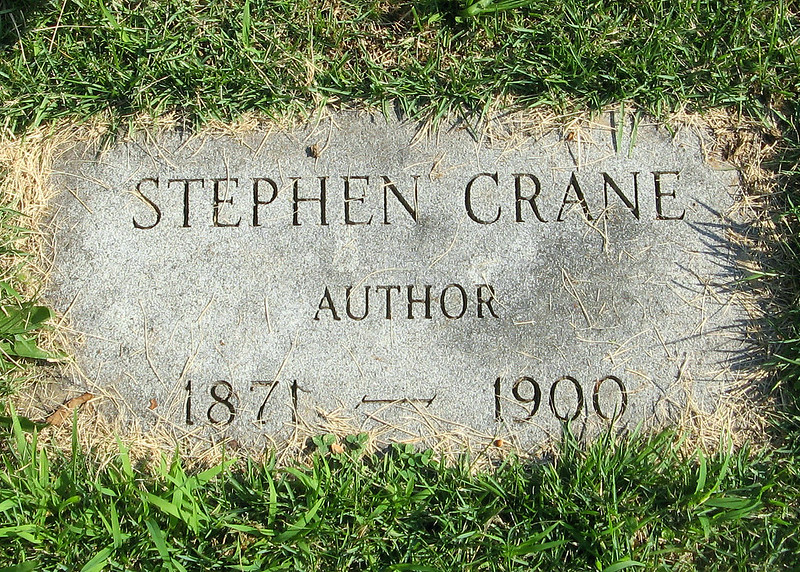
\includegraphics[width=12cm]{Figures/ccby.jpg}
\end{center}
\caption{``\href{https://openverse.org/image/110032f8-1a7a-421f-86b1-88fdfde2e44f
  }{Stephen Crane, Author, Red Badge of Courage}''
  by~\href{https://www.flickr.com/photos/tonythemisfit/}{Tony Fischer
  Photography} is licensed under
\href{https://creativecommons.org/licenses/by/2.0/}{CC BY 2.0}.}
\label{fig:ccbypic}
\end{figure}

The permission can also be from the publisher. For instance, IEEE and
many other publishers have an automated system for granting permission
for theses. Mark the permission in the caption as requested by the
right holder, e.g., “\textcopyright 2022 IEEE. Reprinted, with
permission, from [x].''

Not all figures exceed the threshold of originality. These include,
for example, scientific diagrams and flowcharts. Good research
practices require that even in this case, the source is cited in the
caption (\enquote{Figure from [x].}). However, it would be best to ask
for permission or at least redraw the image. Images with a CC license
are free to use, so long as the terms of use are
followed~\cite{about_cc_licenses}. Even then, the caption must mention
the source (article, website, etc.) and that the image is CC-licensed.

Based on the right to quote, it is possible to take a photocopy,
screenshot or photograph of a work (not the original file) and publish
it, citing the original source in the caption. A critical aspect of
the right to quote is that the use of the image is relevant to the
work, i.e., the image must be related to the subject, and it must be
explained in the text (this applies to all images). Similarly, the
source must be cited in text citations.

Sometimes you may want to use someone else's original image idea as a
basis for your own work. Permission is not required provided that your
work clearly an amply edited version of the original. However, in
accordance with good research practices the type of modification and
source (``Modified/Adapted/Redrawn/Based on/Created using data from
[x]'') and must be declared in the caption. Should you only make minor
edits to the original, separate permission is required. The University
of Oulu Acta Oulu publishing guide~\cite{ronkainen_copyright} has more
details on this topic, and also the proper wordings in
Finnish~\cite{ronkainen_tekijanoikeus}.

When searching for images through an internet image search, it is not
always easy to find the rights holder from whom to request permission
for use. Hunting for a permit can be a demanding task. The easiest way
is to use images and figures from scientific articles (or with open
licenses) as in these the rights holders are clearly declared.

\section{Accessibility}
\label{accessibility}
Put effort into the accessibility of your thesis. The
structure of an accessible document is clear, and the wording is as
understandable as possible. Figures and tables should be given an
alternative text that summarises the information they contain for the
reader. Alternative text is especially important in situations where
the reader cannot see the figure or table, for example due to vision
impairment.  More information on accessible Word documents and
archivable PDF files can be found in the texts of the University of
Oulu Campus ICT~\cite{ictaccessibleword,ictwordpdfa}. You can also
read about the accessibility of mathematical equations in the Campus
ICT text~\cite{ictaccessiblemath}.

    
    \chapter{The literary structure of a thesis}
        \label{experiments}
        % Discussion Chapter

The structure of a text is based on a pre-designed content structure (table of contents and the body) that can vary a great deal from thesis to thesis depending on the topic as well as the scope of the thesis. The presentation order of the first few pages is fixed, and should be presented as it is described in Sections~\ref{sec:first_pages} to~\ref{sec:appendices} in these instructions. When applying page numbering, the title page has page number ‘1’, but page numbers are shown (at the right upper corner of each page, Arabic numerals) only from \charef{introduction}, Introduction, onwards.

\section{First pages}
\label{sec:first_pages}
The first pages include the title page, abstract(s), table of contents, foreword and list of abbreviations and symbols. 

\subsection{Title page}

In case the title page template of these instructions can't be used, you can produce the title page yourself following the model available from the degree program web pages. Please ensure that there are no typos, and that your degree program is stated correctly. Your name should be written into the middle. The title should be written below your name with capital letters, centered, and divided into several lines as necessary to produce a balanced appearance. University logo and the faculty name are placed at the top and the type of the thesis, degree programme name, and date are placed at the bottom.

\subsection{Abstract}

The abstract of your thesis will be fed into various databases and catalogues. It should crystallize the essence of your thesis. A good abstract is a bait that attracts the reader to take a closer look of the content. The abstract should be self-contained, i.e., the reader should be able to get a clear picture of your thesis from the abstract alone. There must not be any references to your thesis or other sources, but it should also not include any information not found in your thesis. The abstract should include the main elements, as well as the methods used and results obtained, and main conclusions of your thesis. The recommended length of an abstract is 200 words. Rare terminology and abbreviations should be avoided. 

The bibliographic information of the thesis should be printed at the top of the abstract page. The keywords of your thesis should be printed below the abstract. The recommended number of keywords is 2--6 keywords or word sets. It is recommended that the keywords are not any words included in the title of the thesis. Keywords serve an important purpose for anyone performing literature searches in a library and other information catalogues. An example abstract is presented in Appendix 1.

\subsection{Abstract in finnish}

You also have to write your thesis abstract in Finnish, or have your abstract translated into Finnish. It should be written in flawless Finnish. If the language of the thesis is English, the abstract in English is placed first, and abstract in Finnish (Tiivistelmä) after it. If the language of the thesis is Finnish the order is opposite. The requirement of the Finnish abstract does not apply to international master’s degree students.

\subsection{Table of contents}

The table of contents lists the chapters with their headings and subheadings and their respective page numbers. However, the page number is shown in the table of contents only from the first chapter, Introduction, onwards.

\subsection{Foreword}

The foreword page should describe the aim of the thesis, and its various research stages, and present the partners, funding and circumstances involved in the thesis project. The forewords should also include words of gratitude, addressed to people who have been incremental in your thesis-writing process. The supervisor, the second examiner, and the technical supervisor can be mentioned as well.

\subsection{List of abbreviations and symbols}

All abbreviations and symbols used in the thesis have to be listed on this page. Abbreviations need to be explained in text as well, when they are used the first time. You should check the validity of all abbreviations and symbols from reliable sources. Concerning measurement units, you should apply the internationally approved SI-system of symbols~\cite{siopas, systemofunits} and quantities and units specified in the IEC 80000-13 standard. For example, 1000 bytes is one kilobyte (1 kB, `B' is Bytes, `b' is bits) and 1024 bytes is one kibibyte, 1 KiB. Similarly, 1 048 576 bytes mebi (Mi); the larger units are gibi (Gi), tebi (Ti), pebi (Pi), and exbi (Ei).

In the list, the abbreviations are defined first, then mathematical and other symbols and last letter symbols so that Latin, Greek and other letters are each presented in their designated groups. 

\section{Introduction}

In the introduction, you should describe the background and motivation of your thesis, introduce the reader to your research questions and methodology, describe in detail the objectives of your thesis (i.e. what is your aim to achieve), and on what basis the scope of your research area has been chosen. You can also state explicitly what will not be covered. You should cite earlier work done in the field. You should \textbf{not} discuss the results of your thesis in the introduction.

You can start by introducing some need of an individual user or the society, or some well-known application or technology. Specifying your own topic as part of such larger entity helps the reader to understand the work and estimate its significance and success. Note that you should avoid specifying too challenging objectives, as failing to meet the objectives can reduce the grade.

Nowadays master’s theses in engineering are often a part of wider research projects at universities or industries, and it might therefore be difficult for the reader to discern when the author is describing her/his personal work, and when is she/he describing the work of a research group. In cases like these, the author should describe as well as possible what exactly was her/his role and contribution in the research/project. At the end of the introduction, you might want to give an overview about the structure of your thesis.

\section{Core text part of your thesis}

How you handle the core topic of your thesis depends essentially on the nature of your research/project. Most theses first describe the technological and scientific environment of the thesis and state-of-the-art related to the topic. This part should focus on presenting context for the author’s own work and for the decisions made by the author, so that it is later clear why one approach, technology, or method was chosen over another.

When the author develops a part for a larger system, it is necessary to describe this larger system as well. For example, when an author develops a software component for an LTE base station, the base station and LTE telecommunication network need to be described. However, the author needs to pay attention to describe the larger system only at a reasonable level of detail. The rule of thumb is that detailed information should be given only when this information is necessary to understand the rest of the thesis.

In the beginning, you can describe and analyze optional approaches or methods, e.g., by applying system-level modeling. As stated above, you can also present solutions proposed in literature sources. The best grades require presenting the state of the art of both technology and science---that is, presenting both the already available solutions and the ongoing research. Such presentation shows that the author possesses good knowledge on the thesis’ topic. Hence, it is crucial to get familiar with the latest literature on the thesis’s topic as soon as possible. Books, scientific articles, and patents can be searched from the sources offered by the university library. The library’s subject guide on information technology\footnote{ http://libguides.oulu.fi/c.php?g=58694} is a good starting point for searching literature.

A theoretical approach on the given topic can become a natural element in some theses where the student presents, based on his on her own prior knowledge or referring to literature, the theoretical grounds on which the
thesis work relies. However, unnecessary wordiness must be avoided and as a result the theory presented must be directly linked to the realised work. It is noteworthy, that many theses do not include a theoretical section of any type. \textbf{Hence, you should not insist on adding theory if itdoes not fit in naturally.}

In the possible presentation of related theory, equations and
mathematical notations often play a prominent role. However, it is
important to keep in mind that mathematics is a tool for technical
writing – not the main purpose. Therefore, introducing all details
with a mathematical equation is unnecessary. It is sufficient to
present the basic equations, necessary variables and the end
results. If needed, the full derivation can be added to the thesis as
an appendix. In science and technology, two types of equations are
employed:

\begin{itemize}
\item{equations between quantities where letter symbols represent physical quantities, and}
\item{equations between numerical values where letter symbols represent the numerical values of the variables.}
\end{itemize}

A quantity is the product of the numerical value and the unit of
measure. The unit of measure must always be separated from the
preceding numerical value with a spac (e.g., 5 Gbit/s,  5\,$^\circ$C, yet 5$^\circ$).
quations between quantities are recommended because they are not dependent on the choice of units of measure, unlike equations between numerical values. Calculations with quantities follow the rules of algebra, and the utilized symbols are typically single letters. The mathematical variables and symbols of quantities must be italicized, i.e., written in italics (e.g., area $A$, electric charge $q$). Vectors must be italicized and boldfaced (e.g., acceleration $\mathbf{a}$).
Numbers, functions, chemical symbols, units of measure, and subscripts are not italicized (e.g., 200, $\cos$, $\log$, NaCl, $\mu$A, cm, electron mass $m_\mathrm{e}$), but subscripts representing symbols of quantities are italicized (e.g., thermal velocity $v_\mathit{T}$). The lowercase Greek letters used as symbols of quantities are italicized, but uppercase letters are not italicized (e.g., $\delta$ vs.\ $\Delta$). More instructions for writing symbols can be found in the SI Guide~\cite{SIguide}, and some of them may be discipline-specific.
List the symbols in the list at the beginning of your thesis, stylized the same as they appear in text and equations. Each equation must be part of a complete sentence. A blank line is left above and below an equation, and the equations are numbered in an increasing order through the entire text or, alternatively, by chapter if there are large quantities of equations. The corresponding order number is placed in parentheses on the right side of the equation. In the text, the equations are referred to by the order number of the equation in parentheses.
In steady movement, speed $v$ is
\begin{equation}
    v = \frac{s}{t},
    \label{eq:speed}
\end{equation}
where $s$ is the distance and $t$ the time travelled. The implications of equation~\eqref{eq:speed}, in turn, are\ldots

Following the first sections of your thesis, your individual contribution will be presented, although parts of it may also be included in the preceding sections. Typically, you proceed with your topic by first introducing the implementation — device construction, electronic circuit, measurement solution, manufacturing method, or similar — together with the rationale and justifications for the chosen solutions. Next, you can present measurement or simulation results, among others, as well as observations aimed at clarifying the functionality of the implementation. To make the observations useful for others, the details of the implementation work must be described accurately, and the observed results must be presented in their original format (for instance in a table). Special attention must be paid to keeping actual results and own estimates separate. In addition, it must be clarified which data results from simulations, and which is produced by measurements.

In a thesis based on a construction or software, the solution is expected to be approached with the means of system planning. Only the essential details, which are of importance for the built device or software, should be given on basic theory and the construction. The exact structure of a device or software can be illustrated in the appendices, if needed. The functionalities of the system are described section by section starting from the largest level towards smaller ones.

When introducing electronic circuits and software structures, you must avoid excessive details. However, in the thesis core, it is justified to present especially such relevant circuit-level structures, which are not self-evident even to experts.

Measurements are intrinsically related to theses which present constructions and therefore they must be carefully planned. The same is valid for the testing of software solutions. Yet, the thesis is not a measurement report and hence it is unnecessary to introduce all the results. Consequently, each presented figure must have a clear significance.

These instructions give guidelines on writing the core text of your thesis when your topic is to develop a concrete solution that can be tested, like a device, piece of software, or an algorithm. Even if the work does not produce such a concrete result, the analytical problem solving has to be present in the documentation and the result be presented clearly. For example, for a literature study, presenting the subject matter and the essential content found from the literature is not enough, but the author has to classify this content or otherwise analyze it. In topics not producing concrete results, such analysis is a mandatory requirement for the best grades. Specifically, it is always crucial to analyze how well the results meet the objectives set in the introduction. This analysis can be placed in the discussion chapter.

\section{Discussion}

A good thesis or other scientific work always has a discussion. In order to write this, you should be able to look at your work as if from a distance, to \enquote{step out of the box}, as they say. You should be self-critical, compare your work to similar work in the field, and think analytically. You should be able to crystallize the results of your work, and put them into words. This can often be difficult even for an experienced writer, but it helps if you are well acquainted with published literature in the field.

A justified analysis of meeting the thesis’ objectives is an important part of the discussion, and generally analysis of the results. When the requirements for the developed solution are presented earlier in the thesis, it is natural to first discuss how these requirement were fulfilled and from that conclude how well the objectives were met. Own solution should also be compared to the state of the art (technology and science) presented at the beginning. Your solution does not have to be better, but this kind of analysis is essential in engineering work and hence an important part of master thesis as well. Such a comparison is needed for the best grades.

The analysis can contain also more general commenting, for example, what was easy and what was difficult in the work. You can also discuss the overall significance of your thesis on a more general level. Outlining potential further development based on your thesis, is valuable, especially if you have put forth clearly new or groundbreaking ideas. However, you should avoid unnecessary speculation here, as well as elsewhere: all statements should be well reasoned and brief. Other requirements for discussion can be found from the supervisors’ evaluation instructions that are available at the degree programme web pages~\cite{mscstudies}.

\section{Summary}

In the summary (or conclusions) you should present clearly in a nutshell the objectives of your thesis, its main content, your results, and the significance of your results. You should lay special emphasis on your results if you feel you have accomplished something. In summary you should not make references, or present any results not found elsewhere in your thesis.

The abstract and the summary overlap to a certain extent; they both describe the main contents and results of a thesis. However, the nature of the summary is broader and it does not have to be self-contained. In it, you should describe your aims, and you could describe any optional solutions or approaches, and motive the choices you have made. The abstract on the other hand could just describe in detail the solutions and approaches chosen for the thesis, leaving the optional approaches out.

\section{References}

The use of references serves many purposes. Scientific method relies on familiarizing with the topic and state of the art. However, efficient referencing can also compress your text, as you can leave the details in the references and repeat only the most important results.

The literature survey should be close to exhaustive, and this means that most of the information you present is taken from references. If a piece of information is not derived or devised by you, it is borrowed, and the origin of the information must be stated. Presenting somebody else’s finding as your own is a scientific theft (plagiarism) that has serious consequences.

You should refer to original sources of the data---for example, to a book and not the handouts made based on the book. Be careful when referencing: the things you state really need to be found from the reference.

The references are mostly cited in your own words, and direct quoting is used only if you want to emphasis the source. In this case you place the quote in hyphens, for example saying that the original phrasing of Moore’s law is  “The complexity for minimum component costs has increased at a rate of roughly a factor of two per year (see graph on next page). Certainly over the short term this rate can be expected to continue, if not to increase. Over the longer term, the rate of increase is a bit more uncertain, although there is no reason to believe it will not remain nearly constant for at least 10 years.”~\cite{moore}.  Correct referencing is  important as the archiving of electronic makes them easily accessible (either in library or in the Internet, depending on the publicity level selected by the thesis author).

The sources are cited and the bibliography is compiled according to
the IEEE model~\cite{ieeetransactions}.  Sources are numbered in
increasing order and listed in the order in which they appear in the
text. The initials of the author's first names are written first,
followed by the last name. References in the text are then indicated
with a reference number, e.g.,~\cite{lappalainen}
or~\cite{lappalainen, acta, korpela}. References to books should
also include page number, for example~\cite[p.~15]{lappalainen}
or~\cite[pp.~15--17]{lappalainen}.

When the reference relates to the content of a single sentence, the
reference is added to the end of the sentence in question prior to the
period. If, on the other hand, the reference refers to the information
presented in the entire paragraph, the reference is placed at the end
of the paragraph after the period of the last sentence. To refer to a
specific page or pages, figure, equation, etc., the formatting
is~\cite[p. 14]{lappalainen},~\cite[pp. 14--15]{lappalainen},
\cite[Fig. 3]{lappalainen} or \cite[eq. (3)]{lappalainen}.

Referencing is easiest to do using \LaTeX\ for writing the thesis and
following the model given in these instructions. You should add your
own references to the file \textit{citations.bib}. A bibliography
manager, such as Zotero~\cite{zotero,uniouluzotero}, is strongly
recommended, as it often automatically fills in the required fields
of the references. 

References need to be presented so that it is clear what information is from a source and what is created by the author. Also the sources of equations, figures, and tables need to be given, when not created by the author her/himself. In addition, permissions need to be asked for tables and figures. Special attention needs to be paid to web sources, as web content can have a short life cycle. Hence, the date of downloading referenced web content should always be mentioned in the reference.

Examples below illustrate correct references. All authors should be listed, the names of journals and series should be written completely without abbreviations, and only the first letter of the title and proper nouns in the title should have uppercase letters. The DOI (Digital Object Identifier) of the publication should be included in the reference, when possible. This identifier locates the publication in an unambiguous fashion and hence facilitates the work of a reader searching the reference. The DOI can be found from the publications front page or from publishers’ databases (e.g. IEEE Xplore, Springer Link, ACM Digital Library).

The \textit{citations.bib} file in Overleaf ITEE MSc thesis template should guide you to use correct citation formats. If you are using other text preparation tools such as Microsoft Word, you should cite articles in journals  as~\cite{ojala:2002}, in series as~\cite{riekki:1998}, and in books as~\cite[p. 55]{pietikainen:2011}. A section of compiled work should be cited as~\cite{cvejic:2005}, and articles in conference proceedings as~\cite{heikkila:1997}. The citation to a thesis should look like~\cite{heikkinen:2011}, and patents should be cited in the manner of~\cite{toivonen:2004}. In some cases it is necessary to cite a source in the Internet~\cite{korpela}, and publications that lack a known author~\cite{asuntoliitto_asumistaso_1969}. Please, see the References Chapter for the models.

\section{Appendices}
\label{sec:appendices}
Things you can include as an appendix are, e.g., derivations of equations or formulas, details of important computer programs, various tables, or performance characteristics and descriptions of special equipment or components applied in the thesis work. You can also include construction drawings and parts of catalogues in the appendix. Appendices are titled as shown before. As with figures and tables, all appendices you include should have a clear meaning---the number of appendices itself is not a merit.

If your text seems to contain a lot of references to an appendix, it may be easier for the reader that you copy the information (e.g., a schematic) into the text. This way the reader does not need to browse between pages.

Large block diagrams or schematics can be copied on A3 size paper. This needs to have two bends (Z-like) so that the right side of the appendix lies top and with a width of ca 2/3 of A4 page.

    
    \chapter{Summary}
        \label{summary}
        These instructions describe the various stages of writing a master’s thesis. We have presented the role of a Master's thesis in an engineering degree, and we have discussed about the importance of keeping close contact with your thesis supervisors. We have also described the procedure, according to which a master's thesis in degree programmes at ITEE, is to be written.
    
    \printbibliography[heading=bibnumbered, title=\mybibname]

    \startappendix
    \chapter{Appendices}
        % Appendix Chapter

Appendix 1 \hskip 2.5em Example Abstract 
\vspace{7em}

\noindent Note 1: Page numbering is done by consecutive numbering. Additional appendices, that are attached to the thesis (such as copies, drawings, etc.) are left without page numbers and placed at the end of the thesis.

\newpage
\markboth{left}{\normalfont{Appendix 1. Example Abstract}}

\noindent \textbf{Jurmu M.\ (2007) Resource Management in Smart Spaces Using Context-Based Leases.} University of Oulu, Department of Electrical and Information Engineering. Master’s Thesis, 77 p.

\begin{center}
\textbf{\fontsize{16}{19pt}\selectfont ABSTRACT}\\
\end{center}

{\bfseries \noindent The convergence of wireless access networks in conjunction with the increased computing power of the handheld terminals is preparing the emergence of the ubiquitous computing paradigm. In the center of this paradigm are smart spaces, which are local environments saturated with various embedded computational resources. These spaces co-operate with mobile client devices in enabling advanced, service-oriented computation scenarios. This co-operation is typically enabled through the utilization of distributed and modular middleware frameworks. An emerging additional requirement however is the possibility to harness resources from the proximity environment to the mobile device in an on-demand fashion. This is a challenge especially to the resource management infrastructure of the smart spaces.

This thesis explores the concept of a smart space and presents a review of the current research and technologies. Subsequently, a lease-based design for resource management in smart spaces is presented. Leases in this work are negotiated agreements between the mobile clients and the resource management infrastructure, regarding the harnessed resources. Leasing is seen as a suitable solution for the management due to the transient nature of the resource usage. The inclusion of additional contextual features to the leases further facilitates the management.

Requirements for the design are derived from the review and from an example usage scenario. The requirements include dynamic mapping and contracting of resources from the proximity environment, monitoring of the contract validity, access control towards the resources and dynamic maintenance of the smart space infrastructure. Presented design is analytically compared against existing solutions, and several points for future development are listed. According to the comparison, none of the existing solutions utilize contracts with contextual validity in resource management. Two publications of this work have been accepted into an international conference and a workshop on the focus area of pervasive computing.

\lskip \textbf{Keywords: Ubiquitous computing, mobile computing, task-based computing, context-awareness, QoS.}
}

\end{document}
